\documentclass[11pt,oneside,a4paper]{article}
\usepackage{graphicx}
\usepackage{booktabs}
\usepackage{caption}
\usepackage{subcaption}
\usepackage{amsmath}
\usepackage{amsfonts}
\usepackage{amssymb}
\usepackage{lscape}
\usepackage{psfrag}
\usepackage[usenames]{color}
\usepackage{bbm}
\usepackage[update]{epstopdf}
\usepackage[bookmarks,pdfstartview=FitH,a4paper,pdfborder={0 0 0}]{hyperref}
\usepackage{verbatim}
\usepackage{listings}
\usepackage{textcomp}
\usepackage{fancyhdr}
\usepackage{multirow}
\usepackage{tikz}
\usepackage{lipsum}
\usepackage{xcolor}
\usepackage[margin=1in]{geometry}
\newcommand{\hint}[1]{{\color{blue} \em #1}}

\makeatletter
\def\cleardoublepage{\clearpage\if@twoside \ifodd\c@page\else%
\hbox{}%
\thispagestyle{empty}%
\clearpage%
\if@twocolumn\hbox{}\clearpage\fi\fi\fi}
\makeatother

\sloppy
% \widowpenalty=10000
% \clubpenalty=10000

\title{
    \vspace*{0.0mm}
    \LARGE\bf\sf Advanced Topics in \\Communication Networks (Fall 2019)
    \vspace*{10.0mm} \\
    \Large\bf\sf Group Project Report \vspace*{30.0mm}\\
    %
    \Huge\bf\sf Hearding the Elephants: Detecting Network-Wide Heavy Hitters with Limited Resources
    %
    \vspace*{30.0mm} \\
    \normalsize
    %
    \sf Authors:\\[5pt]
    \sf Yannick Merkli\\ [5pt]
    \sf Tim Bohren\\ [5pt]
    \sf Felix Rüssli \vspace*{5mm}\\
    %
    \sf  Advisor: Albert Gran Alcoz \vspace*{5mm}\\
    %
    \sf  Supervisor:  Prof. Dr. Laurent Vanbever \vspace*{20.0mm}\\
    %
    \sf Submitted: Dec 16, 2019\\ [5pt]
    \sf \pageref{lastpage} Pages
}
\date{}

\begin{document}

\begin{figure}
    \includegraphics[width=\textwidth]{figures/eth-nsg-header}
\end{figure}

\maketitle
\thispagestyle{empty}
\raggedbottom
\clearpage

\pagenumbering{roman}

\begin{abstract}
Detecting heavy hitters (e.g. flows whose packet counts exceed a certain threshold) is an important task for Denial of Service detection, load balancing and traffic routing. Past work has shown how to detect heavy hitters on a single network switch. However, nowadays heavy hitter flows are often \textit{network-wide}, thus detecting them on a single switch is not enough. A flow can enter a network over multiple ingress switches and from each switch's local view, the flow might look like normal. However, from a global view, the flow would be classified as a heavy hitter. A detection protocol should \textit{quickly} detect flows from a \textit{global view}. Further, detecting heavy-hitter flows inherently poses a trade-off between limitations in network-wide communication and memory resources on the ingress switches and accuracy in detecting heavy hitters. 

In this work, we have implemented Herd \cite{anon2019herd}. Herd is a distributed algorithm that identifies network-wide heavy hitters in real time and under constraints on communication and switch memory. The algorithm uses a sample-and-hold technique for flow measurements on ingress switches and probabilistic sampling and reporting of flows. Reporting is done to a central coordinator, which allows for a global view on the network.

\end{abstract}

\clearpage
\setcounter{tocdepth}{2}
\tableofcontents
\clearpage
\pagenumbering{arabic}

\section{Introduction}

Heavy hitters are a minority of flows that are responsible for a majority of packets inside a network. Network operators are interested in spotting them in order to detect and prevent Denial of Service attacks and to maximize the throughput by detecting congestion and failures. Further, heavy hitter detection can also be used for network management such as usage-based pricing or load balancing. To effectively manage and protect networks, heavy hitter detection needs to be quick and efficient. For the following sections, we assume a network to consist of multiple ingress switches through which traffic enters a network. The topology of the inner network is ignored and not important for this work.

Detection of heavy hitters faces several challenges. First of all, heavy hitters don't necessarily enter a network through a single ingress switch and they don't always originate from a single source. As an example, a single host inside a network might be the target of a denial-of-service attack, but traffic targeted towards the host may enter over multiple ingress switches. Local detection on ingress switches will not capture the network-wide view of a flow and will inherently fail at detecting network-wide heavy hitters. Second, network devices are usually limited in their resources, especially when it comes to memory and processing power. This often results in network operators having to choose between high detection accuracy and low processing overhead (i.e. low delay).

\noindent The problem of a missing network-wide view can be solved by introducing a centralized instance that receives and aggregates partial information from network devices. The burden of heavy hitter detection thus no longer lies on ingress switches but on this centralized instance; usually a general-purpose CPU. The ingress switches only observe and report flows.

\noindent With unlimited memory and processing power on switches and unlimited communication, detecting network-wide heavy hitters would be easy. Each switch could keep track of every single flow, communicate as much as needed with the centralized instance, which can immediately detect based on aggregated information. In reality, switches are highly limited in their memory and processing power. Sending a subset of flow information to a central, general-purpose CPU lifts parts of the limitations on processing power and memory, however new limitations are introduced by the resulting network-wide communication and the fact that a general-purpose CPU is not able to process data at line rate.

%brief description of Herd
Herd \cite{anon2019herd} solves these problems by sampling traffic probabilistically, which saves memory on the switches, and reporting to a central coordinator once an observed flow exceeds a certain threshold. This allows for high accuracy in flow detection while operating under the constraints imposed by network devices. The coordinator sees all flows that entered the network and that were reported by an ingress switch. The coordinator is thus able to combine partial information reported by various ingress switches. This system makes it possible to not only detect local heavy hitters, but also distributed ones, potentially even detecting distributed Denial of Service attacks (DDoS) before they grow to their full potential.


\section{Background and related work}

The basic problem to solve is the following: various flows enter a network and we want to classify them based on a measure that captures each flow's strain on the network (e.g. the packet count). We then want to distinguish \textit{mice flows} (flows without local or global significance) from \textit{elephant flows} (flows with local and global significance). 

There already exist a number of protocols with different approaches to detect elephants. Some existing algorithms, such as NetFlow \cite{claise2004netflow}, sample incoming packets and export them to a central collector. This addresses the constrained switch resources and the flow locality, however these algorithms suffer from temporal 'blind spots' due to low sampling rates and the resulting long delays. Other approaches to heavy hitter detection run streaming algorithms, combined with a compact data structure like a count-min sketch \cite{cormode2003countmin} or a bloom filter. 

These algorithms address the resource constraints of switches, however they fail to capture network-wide heavy hitters since detection is done on each switch individually.

\begin{figure}
	\centering
	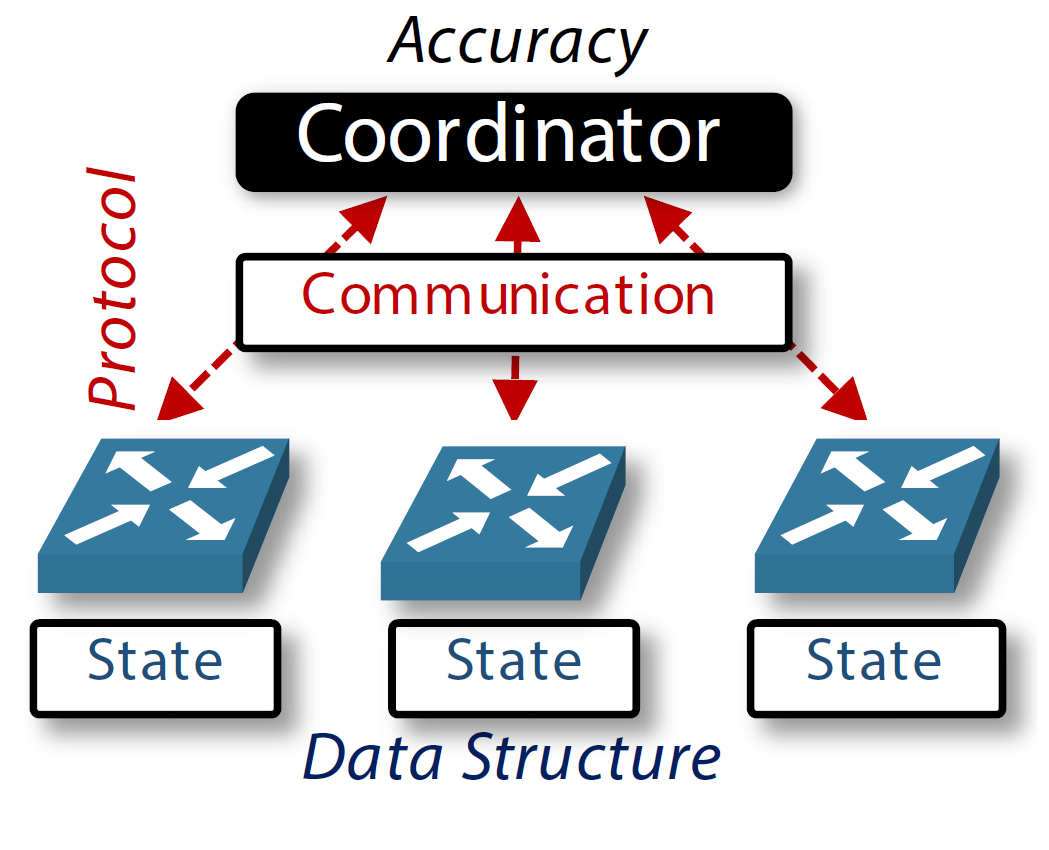
\includegraphics[width=0.5\textwidth,scale=1]{figures/global_local_paper}
	\caption{The Herd switches communicate with the coordinator. \cite{anon2019herd}}
	\label{fig:global_fig}
\end{figure}

\section{Implementation}

We have implemented Herd, as proposed by \cite{anon2019herd}. The Herd architecture consists of local ingress switches and a central coordinator that achieves a global view. Ingress switches probabilistically sample and report incoming flows to the coordinator.
Each flow can be of local and global significance. Additionally to mice and elephants, Herd thus introduces two more flow categories to describe all four types of significance: mice, moles, mules and elephants.

\subsection{Herd algorithm} \label{animals}

All flows that enter a network are first classified as mice (a flow is defined by the five-tuple $(srcIP, dstIP, srcPort, dstPort, protocol)$). Mice are the most common but also the smallest flow type. When a packet arrives, Herd uses the sample-and-hold algorithm: if the flow to which the packet belongs is already tracked, then its counter is simply increased. Otherwise, we start tracking the flow with sampling probability $s$. With an increasing number of packets belonging to the same flow, the flow's packet count is more likely to be tracked.

\noindent Once a flow is captured by an ingress switch it advances to the next higher tier: the mole. A mole flow is simply a flow whose packet count is tracked by an ingress switch. As such, a mole flow exhibits local significance but no global significance.

As soon as the packet count of a mole flow on a single ingress switch exceeds the mule threshold $\tau$, the mole flow is reported to the coordinator with report probability $r$. The packet count threshold $\tau$ is introduced for two reasons: First, the coordinator should not waste its precious memory on every mouse flow that happened to be sampled by the switch. By making sure that each reported flow's packet count exceeds a certain threshold, we ensure to only report globally significant flows that have the potential to  become an elephant, especially when combining reports for the same flow from multiple ingress switches. The other reason is that the network does not have infinite bandwidth, so the switches have to be careful not to congest the links with coordinator communication. A flow that has been reported to the coordinator at least once advances from mole flow to mule flow, which means that the flow now has global significance.

\newpage

The coordinator has a global view over all mule flows reported by the ingress switches running Herd. In contrast, the ingress switches only have a local view since they do not know what other switches observe. Thus the actual classification of elephant flow is solely done by the coordinator. It counts how many reports for a specific flow were received, independently from which switch the report originated from, and as soon as the number of reports for a mule flow exceeds $R$ the coordinator classifies the flow as an elephant flow, which is synonymous to being a heavy hitter.

\begin{figure}
	\centering
	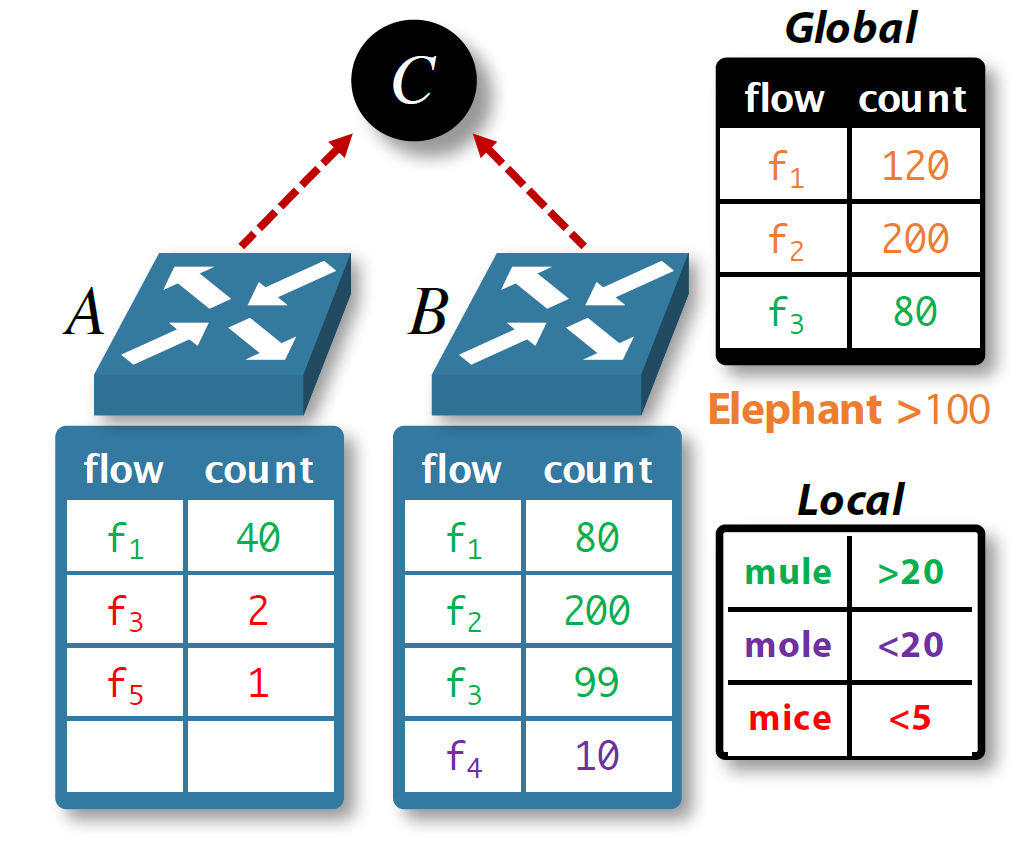
\includegraphics[width=0.5\textwidth, scale=1]{figures/paper_zoo}
	\caption{Zoology in the Herd protocol.}
	\label{fig:zoo_fig}
\end{figure}

\subsection{Locality} \label{locality}
So far it was assumed that all ingress switches have the same probability to observe a flow. However, in real networks flows often exhibit preference for certain ingress switches. So, certain switches are more likely to observe certain flows. Considering this, we need to increase the mule threshold $\tau$ since every ingress switch observes more packets for fewer flows. A too low mule threshold $\tau$ would result in too many flows being reported to the coordinator, which increases the network-wide communication and increases the number of false positives.

Herd thus introduces the notion of a \textit{locality parameter} $l_f$, which denotes the number of ingress switches that observed flow $f$. However, tracking the locality on a per-flow level introduces significant overhead. That's why Herd only tracks the locality on a per-group level. A group is defined as

$$g_{src,dst} = \{f | f.srcIP \in src, f.dstIP \in dst\}$$

\noindent where $src$ and $dst$ are /8 IP subnets.

\noindent The new locality parameter $l_g$ now tracks how many ingress switches observe a flow $f \in g$. Using the per-group locality parameter $l_g$, the mule threshold $\tau_g$ and the report probability $r_g$ can now be dynamically adapted on a per-group level. Since tracking $l_g$ requires a global view of the network, this is done at the coordinator. For the coordinator to know which ingress switch observes which flows, the ingress switches need to send a message to the coordinator when observing an unexpected (i.e. never before seen) flow. These messages are called \textit{hellos} in Herd.


%Herd tracks the locality $l_f$ of a flow $f$ dynamically. If the ingress switch encounters a unexpected flow $f$ it sends a message to the coordinator. The coordinator then updates internally which switches see the flow $f$ and reports back to the switch with $l_f$. Of course the coordinator also has to inform the other switches which observe $f$, but it only does that once the number of observing switching has doubled to save on bandwidth.

\subsection{Switch logic} \label{switch}
Herd uses randomness for packet sampling and reporting to the global coordinator. Since P4 doesn't have a random library, hashes are used to 'flip' coins and simulate randomness. A  32bit hash $h$ is calculated from timestamps, the destination IP and the last hash; if 

$$h < int32_{MAX} * probability$$

\noindent the probability is hit. However, the right part of this inequation requires floating point arithmetic, which P4 does not have. For this reason, the calculation $int32_{MAX} * probability$ is done by the local controller at startup and the resulting \textit{int32} number is then written into a register which can be read by the data plane.

As described in section \ref{locality}, the mule threshold $\tau_g$ and the report probability $r_g$ vary on a per-group level. We thus use a match-action table that maps a group $g_{src,dst}$ to its respective values $\tau_g$ and $r_g$. A second match-action table is used for packet forwarding. As of now, ingress switches simply forward all traffic to an internal aggregator switch, thus this table only has one rule.

The life of a packet when entering an ingress switch looks as follows: the switch first extracts the group $g_{src,dst}$ to which the flow belongs and applies the group values match-action table. In case of a table miss the switch sends a hello message to the local controller, which will then send the hello to the coordinator. The coordinator answers with the locality parameter $l_g$ to the local controller, which will then add a rule to the group values table. For known groups the switch applies the sample-and-hold algorithm. In case the flow is not yet being sampled, we start sampling it with sampling probability $s$. If the flow is already being sampled, its counter is increased. In case the counter reaches the group-based mule threshold $\tau_g$, the switch resets the counter and reports the flow with report probability $r_g$. Again, the report will first be sent to the local controller, which will then send it to the coordinator. The communication between data plane and control plane (hellos and reports) is done via copy-to-cpu, where a cloned packet has a CPU header which has six fields: $(srcIP, dstIP, srcPort, dstPort, protocol, flow_count)$.

The counters counting the number of seen packets per flow are stored in a multi-stage hash table with three stages. The index of the flow counter in the hash table is determined by hashing the flow five-tuple $(srcIP, dstIP, srcPort, dstPort, protocol)$. Register entries are 64 bit wide. The lower 32 bit store the flow count. The upper 32 bit store a hash (with a different hash function) of the flow five-tuple (hash key) which is used to detect hash collision. In case of a hash collision, the next hash table is considered. Note that the width of the registers can be chosen smaller than 64 bit. In case of few flows, hash collision become less likely and a smaller hash space for the flow key is acceptable. Further, the flow counter will never become larger than $\tau_g$ since at that point it will be reset to zero and a report will be sent. We decided to use 64 bit wide registers to make sure that hash collisions are unlikely, even for large numbers of flows.

\subsection{Herd Controller} \label{controller}

A Herd controller is running on each ingress switch. The controller's main task is to communicate with the coordinator and write rules into the group values match-action table.

\noindent During the startup phase, the controller cleans all hash tables, writes the sampling probability to the data plane, fills the forwarding table and connects to the coordinator RPC server. To handle communication between data plane and control plane, the controller sniffs on the copy-to-cpu interface and unpacks each received cloned placket. Each clone packet includes a CPU header, stating the flow five-tuple and the packet count for the flow (flow count). The controller determines based on the flow count whether the received message is a hello or a report: hellos have a flow count of zero whereas reports have an flow count larger than zero. The controller then sends the hello or report by initiating a remote procedure call towards the coordinator, including the flow and the switch name as arguments.

\noindent When a flow belonging to a never before seen group $g$ arrives at an ingress switch, it is possible that the data plane sends multiple hellos due to delayed writes into the group values table. In order to avoid overloading the network with hellos, we adapted the Herd controllers to keep track of the flows for which a hello was already sent. This way, each controller only sends one hello per flow to the coordinator and we don't overload the network or the coordinator with unnecessary hello messages.

Controller-coordinator communication is two-way since the coordinator needs to answer with the locality parameter $l_g$ and respective flow $f$ upon receiving a hello. Additionally to a sending part, the Herd Controller thus also has a receiving part. Upon receival of $l_g$, the controller calculates the mule threshold as $\tau_g = \frac{\epsilon \cdot T}{l_g}$ and the reporting probability as $r_g = \frac{1}{l_g}$. Additionally, $r_g$ is transformed into an \textit{'int32-probability'} (see section \ref{switch}). The controller then writes $\tau_g$ and $r_g$ into the group values table with the group $g$ $(f \in g)$ as match key and $\tau_g, r_g$ 




Due to the delay between the switch sending a hello and the controller writing the group values into the match action table, it is possible that the group values table does not yet have an entry for a group although a hello was already sent. Thus, if the second packet of a flow for which a hello was sent arrives \textit{before} the table write happens, a second hello will be sent to the controller. It is therefore possible that the Herd controller receives multiple hellos for the same flow. 





Whenever an incoming packet on the switch creates a table miss in the group values table, the switch will send a hello. The total delay between the switch sending a hello and the controller writing the table rule is 

$$\Delta t_{hello} = t_{copy-to-cpu} + 2*t_{CC} + t_{table\_write} + \epsilon$$

\noindent where $t_{copy-to-cpu}$ is the delay introduced by the copy-to-cpu, $t_{CC}$ is the delay introduced by the controller-coordinator communication, $t_{table\_write}$ is the time it takes to write $\tau_g$ and $r_g$ into the group values table and $\epsilon$ are negligible processing delays. In case the arrival time of the first packet belo

 




\subsection{Coordinator} \label{coordinator}
The global coordinator handles all the messages sent to it and reports back with new locality parameters to the individual switches if necessary. 

When a hello arrives from a switch the coordinator checks whether the coordinator has already seen the switch or the flow before. If not it saves them. Now the uses the HandleHello function from the original paper. First it checks whether it had already got a hello from that switch with that flow. If not if saves it in the dictionary $S_f$ and finally sends notices all switches in updated $S_f$, but only if the size of $S_f$ doubled in order not to overwhelm the links with update messages. If $S_f$ didn't double in size, the coordinator only sends a notification to the new switch in $S_f$ about the current size of $S_f$.

Handling the reports is quite simpler. The coordinator simply counts the number of reports arriving at it for each flow. And after enough reports arrived the flow get put into a list with all the other heavy hitters. Finally upon shutdown it writes found elephants into a $.json$ file for further processing.

\subsection{Tuning the parameters} \label{tuningparameters}
Until now it was assumed that the parameters $\tau$, $s$, $r$ and $R$ were given. Now we try to find those paramaters in order to maximize the detection accuracy of Herd under communication and switch memory constraints. We do this by simulating the whole protocol for one Herd switch and the coordinator. In tuningparameters.py one can specify the packets needed to promote a flow into a heavy hitter and a set of training data in form of a pcap-file, but also the limited switch memory and communication budget. The program then iterates through the possible approximation factors $\epsilon$ and returns the parameters which maxime the accuracy.

First, we try to configure the sampling probability $s$ of the sample-and-hold algorithm. With unlimited switch memory $S$ the sampling probability could simply be set to $s=1$ and the switches would memorize all flows going through them. Let $M$ be the set of observed moles on the switch. Thus the switch has to store $|M|$ different flows. From this we conclude that we need $|M| \leq S$ in order to be able to store all the observed flows. To be sure that the real $M$ has enough space in $S$ we even want $|M| < S$. In order to have this in expectation $s$ is set to $1/\tau$. For that an estimation of $\tau$ is needed. At the beginning $\tau$ is set to the global threshold $T$. $T$ is the size a flow needs to have in order to be recognized as a heavy hitter. Then we look in our training data $D$ how many moles are found and check whether the found moles $M$ use up all the memory $S$. Afterwards $\tau$ is made smaller to increase the chance to categorize a flow as mole. This is done iteratively as long as there is still space in $S$. 

If unlimited bandwidth was available $r$ could be set to 1, since there would be more than enough bandwidth to send all the mule reports to the global coordinator. Further, the coordinator would need at least $R = T/\tau$ reports to classify a flow as elephant. However, under the communication budget $C$ the parameters $r$, as well as $\tau$ and $R$ need to be adjusted. This is done with the help of the approximation factor $\epsilon$. We approximate global threshold with $\epsilon$ and expect to see at least $\tau$ packets of that flow on every local switch with that flow, so in $l$ switches. This brings us to the equality $\tau l = \epsilon T$, from which we get $\tau =$ $\epsilon T\over l$. Now that we have again a $\tau$. We calculate now first the set of moles $M$ from our training data, and then from that the set of mules $U$ since the necessary $\tau$ is now available for that. The total number of sent reports can be bound with $T|U|r\over \tau$ which leads to $r =$ $T|U|C\over \tau$. The coordinator needs to see at least $R =$ $lr\over T$ reports. We can now finally adjust $\epsilon$ in steps of $\sigma =$ $l\over T$ since $\tau$ is an integer. Every time we change the value of $\tau$ we calculate $\tau$, $r$ and $R$ anew as well. This is done until the accuracy decreases for the first time. Afterwards the program returns the optimal parameters and terminates.

\subsection{Full hash tables} \label{special}%title

Flow counters are stored on each ingress switch in a multi-stage hash table. In case of full hash tables, Herd proposes to just send all packets of the flow to the coordinator. This introduces significant delay and communication cost. In our implementation, we handle full hash tables differently. Instead of sending all packets to the coordinator, the data plane sends an error message to the controller, indicating full hash tables. The controller will subsequently resets the hash tables. We argue that due to the fact that counters of large flows are reset back to 0 anyways in case of a report, this leads to a minor decrease in accuracy.

\subsection{Challenges} \label{challenges}
Since the traffic we received from CAIDA for the evaluation had no MAC addresses we had to append our own created MAC addresses.

The topology for the evaluation needs an additional load-balancer in front of the switches running Herd. This is needed in order to distribute the packets across all the ingress switches from $h1$. 

Additionally the load-balancer has to distribute the flows randomly between two randomly chosen switches. 

At the other end of the ingress switches we had a similar problem. This is why we put an aggregating switch between the ingress switches and $h2$. This switch collects again all the packets from the ingress switches and forwards them to $h2$. 

We faced further challenges with the communication between the ingress switch controllers and the coordinator. Since the communication between those two is asynchronous, for example a report about a mule could arrive at the coordinator before the hello and therefore not be store.%uh... really? I think the example is wrong.

The original paper mentions the implementation of a rolling window which resets the hash tables every $W$ seconds. Further, once all the hash tables are filled the ingress switches were to send every single sampled packet of a new flow to the global coordinator. So basically these new flows would have $\tau = 1$ and $r = 1$. The coordinator would therefore pretty much instantly classify these flows as heavy hitters even if they aren't. We didn't like this solution of the rolling time window since it doesn't solve the problem of what happens to new flows once the hash tables are full. We solved this problem by instantly resetting the hash tables once they can't accomodate a new flow, and therefore not waiting until the window $W$ is closed. Our solution doesn't overflow the coordinator with reports about the new flows.

Further we faced severe speed issues. The scapy library often reached its limit in terms of speed. Another challenge was that the pcap files are often so big that it takes a long time to test the implementation of Herd. This makes the testing process even slower together with scapy. 
%how we solved it. I need to have explained again.
However, the speed issues we faced are only a problem in software, since the speed of the whole architecture in would be a multiple of the speed in software when implented onto hardware.

We also tried digests, however we found that digests are slower which introduces significant delay between the data plane sending a message and the controller receiving it, which leads to an increase in false negatives since the switch misses packets as long as no table entries are written. In real hardware, this would not be an issue since there exists a direct link between data plane and control plane, which allows for diminishing delay. In real hardware, the delay introduced by the communication between controller and coordinator would be would dominate.

\subsection{Assessment of the original paper} \label{original_paper}
Due to the original paper on being only a rejected conference submission and not an accepted paper we faced many challenges along the way. The authors are often extremely vague. For instance the topology used for evaluation is barely mentioned. The paper also contains mistakes. For example in the GetSampling function the sampling probability is not adjusted in the while-loop which could trap the program in an infinite loop. The idea of a rolling time windows sounds rushed. This is why we implemented that the switch resets once the table is full.

%\lipsum[1-5]

\section{Evaluation}
\subsection{Topology} \label{topology}

\begin{figure}
	\centering
	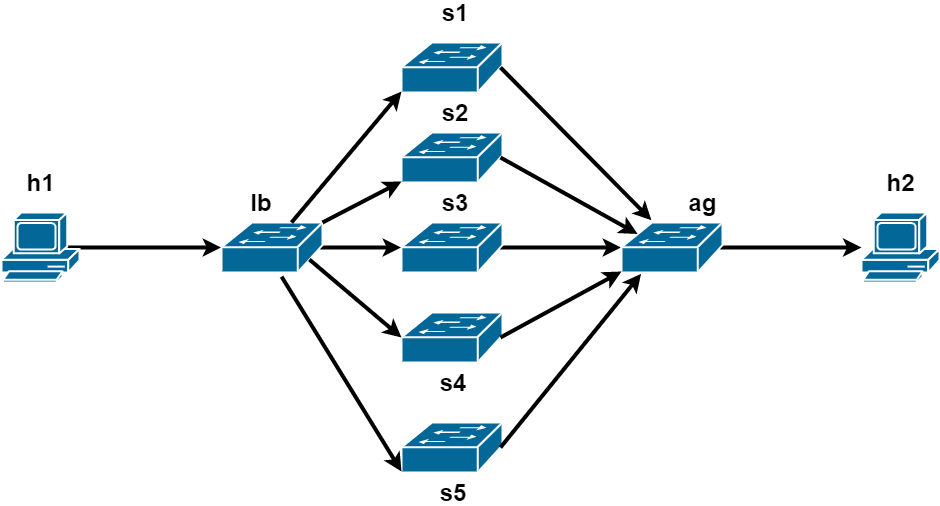
\includegraphics[width=1\textwidth]{figures/Herd_topology}
	\caption{Topology for the evaluation. h1 sends traffic over the loadbalancer, a Herd switch and the aggregating switch to h2.}
	\label{fig:topology_fig}
\end{figure}

As topology we use two host, $h1$ sends the traffic and $h2$ receives it. $h1$ sends to programmable switch $lb1$ which is there for load balancing. $lb1$ fowards the packets to the switches $s1 - s10$, which run the Herd protocol. The ingress switches $s1 - 10$ are an aggregating switch $ag1$ which is finally linked to the receiving host $h2$.\\

We had to separately build a load balancer for our test setup. In order to distribute the flows between the Herd switches the load balancing switch chooses randomly two Herd switches. The load balancer then forwards each packet of the flow to one of the two chosen switches. This has to be done this way since in the evaluation of the original paper each flow has exactly two switches observing each flow. Of course this procedure wouldn't be necessary in a real world application. There the number of observing switches would not be given by a separate switch, but according to the flows themselves, and therefore out of the direct control of the operators. Also the number of observing switches would not be limited by two. The coordinator would then forward this number to the switches according to the algorithm with the hello messages to take the locality of the flows into account.

Since the load balancing and the aggregating switch work differently from the ingress switch they get both their own controller and switch logic.

\subsubsection{Load-balancer}
The load-balancing switch chooses for each flow two random ingress switches and forwards the packets of that flow randomly to one of those two switches.
The corresponding controller forwards traffic to the ingress switches according to their switch ID.

\subsubsection{Aggregating switch}
The aggregating switch simply fowards every received to the end host.
Its controller receives the traffic from all ingress switches with Herd and forwards everything to the endhost.

\subsection{Traffic} \label{traffic}
To generate a sizeable amount of traffic on the sending host $h1$ we use CAIDA's anonymized Internet traces from 2016, like the original paper did. Using the $send.py$ script on $h1$ parses the packets stored in a $.pcap$ file and $h1$ forwards them through the testing topology. Further the script counts how often a packet was sent for each flow and writes flows that were seen more than $T$ times in $real\_elephants.json$ for later comparison with heavy-hitters found with Herd.

Configuring the parameters $\tau$, $r$ and $R$ in isolation might actually impact the accuracy of Herd negatively. Thus $tuningparameters.py$ simulates the whole protocol with given training data in order to reach the best possible accuracy for the running protocol.

\subsection{Evaluation} \label{evaluation}
\begin{figure}
	\centering
	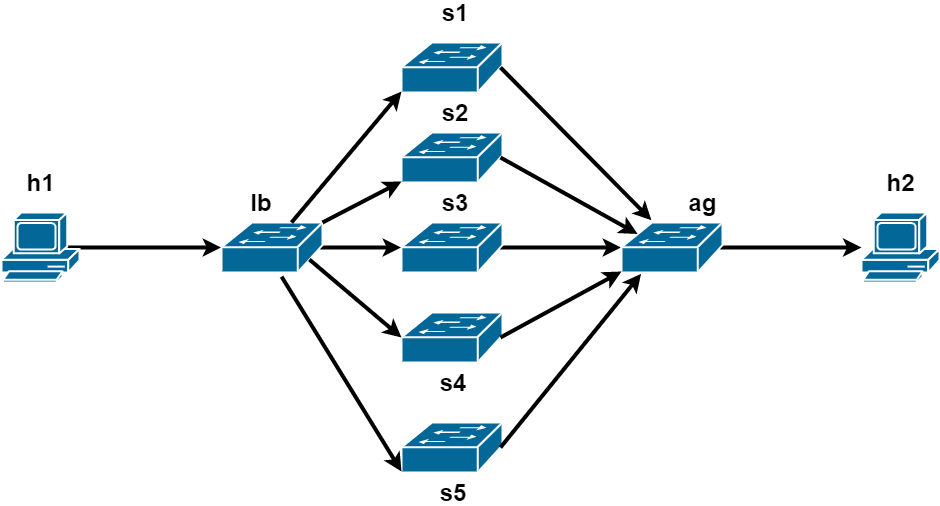
\includegraphics[width=0.5\textwidth]{figures/Herd_topology}
	\caption{some graph about the evaluation}
	\label{fig:topology_fig}
\end{figure}

\lipsum[1]
Something in %\figref{topology_fig}. %I still don't understand how \figrefs work.

\begin{figure}
	\centering
	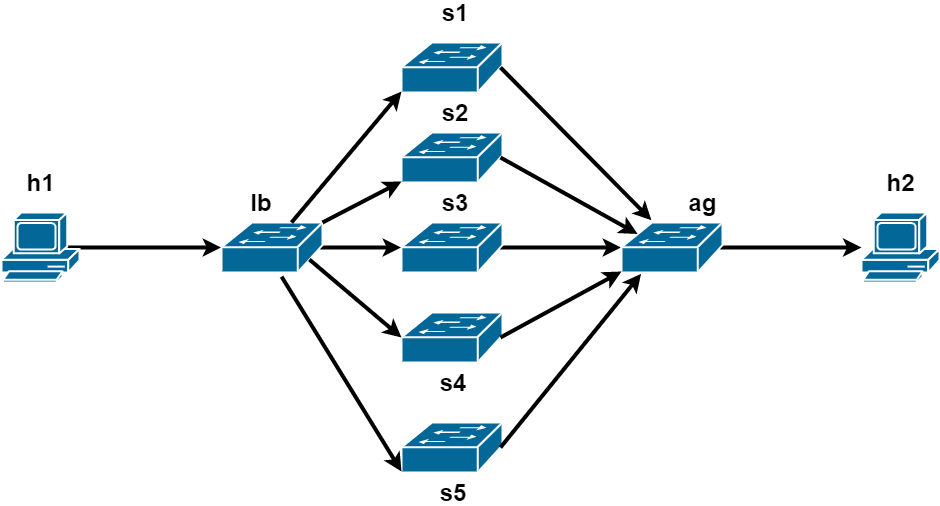
\includegraphics[width=0.5\textwidth]{figures/Herd_topology}
	\caption{some other graph}
	\label{fig:topology_fig}
\end{figure}
%\lipsum[1-2]

\section{Conclusion}
\hint{A brief conclusion about how you solved the project.} \\
We reimplemented Herd, a distributed heavy hitter protocol. Compared to the original paper we changed when to reset the flow/count tables. Further we had to implement a load balancing switch in front of the Herd switches for the evaluation. Additionally, we had severe speed issues in the implementation in software compared to a implementation in hardware.

Further research could go towards improving the selection of the parameters. How it is implemented at the moment, the tuning has to be done ahead of the protocol with training data. An improved protocol could maybe adjust the parameters according to captured data, and not prerecorded data. Even a dynamicaly changing tuning can be imagined. Another research topic would be, in case a single coordinator reaches its limit in processing power and speed, to have multiple coordinators, each responsible for a subnet, transferring data between each other.
%\lipsum[1]

\label{lastpage} % this must stay here
\clearpage
\addcontentsline{toc}{section}{References}
\bibliographystyle{acm}
\bibliography{refs}

\clearpage
\appendix
\pagenumbering{Roman}

\section{Group organization}
\hint{Briefly describe what each team member was contributing to the project}%still a bit lacking

\paragraph{Yannick Merkli}
\begin{itemize}
	\item Coordinator
	\item Controllers
	\item Load balancer, aggregator
\end{itemize}


\paragraph{Tim Bohren}
\begin{itemize}
	\item Ingress switch (P4 part of Herd)
	\item Data plane - control plane communication
	\item Automated evaluation
\end{itemize}

\paragraph{Felix Rüssli}
\begin{itemize}
	\item Tuning Parameters
	\item Report
	\item Presentation
\end{itemize}

\end{document}
